\section{Glyph-based Solutions for File System Visualization}
\label{sec:file_system}
Glyphs are typically small, and are often designed with a high-degree of similarity in order to facilitate mapping consistency, semantic interpretation, learning, and memorisation.
In many applications of spatial or temporal visualization, it is often the case that a large number of small glyphs are displayed on the screen at one time.
For the biological workflows described in Chapters \ref{chap:glyph-tax} and \ref{chap:automacron} for instance, the number of glyphs on the screen can be in the thousands.
In this chapter we are focused on the \emph{differentiability} of such glyphs and solutions to potential perceptual errors in their observation and exploration.

Figure~\ref{fig:reduction_degradation} presents some example cases that may render some glyphs indistinguishable. 
For example, zooming out in data exploration can reduce glyph size significantly.
This could make some shapes (\eg, circle and hexagon) and textures appear similar, while confusing the categorisation of sizes (\eg, big, medium, small).
Additionally, environmental lighting conditions, and printing or photocopying facilities can cause colour and greyscale degeneration.
Such changes would make some glyphs indistinguishable, and also confuse associations between different colours or shades of grey and the concepts they represent.
A dynamic legend may help alleviate the confusion about various mappings, however these legends demand regular attention from users.
This extra lookup action incurs additional cognitive load due to the effort required for visual search and memorisation of unstable mapping keys.
These issues may be compounded by colour- or change-blindness, short- or long-sightedness, clustering, occlusion, and distortion.

\begin{figure*}[t]
\begin{center}
%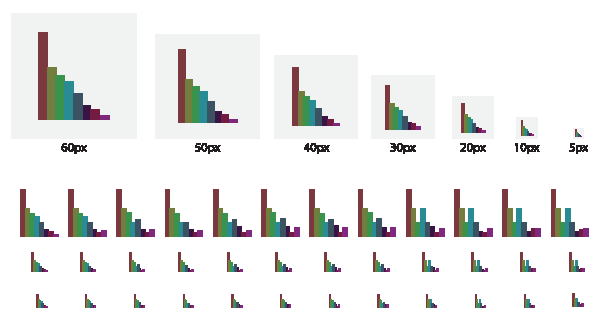
\includegraphics[width=0.9\textwidth, height = 3in]{problems}
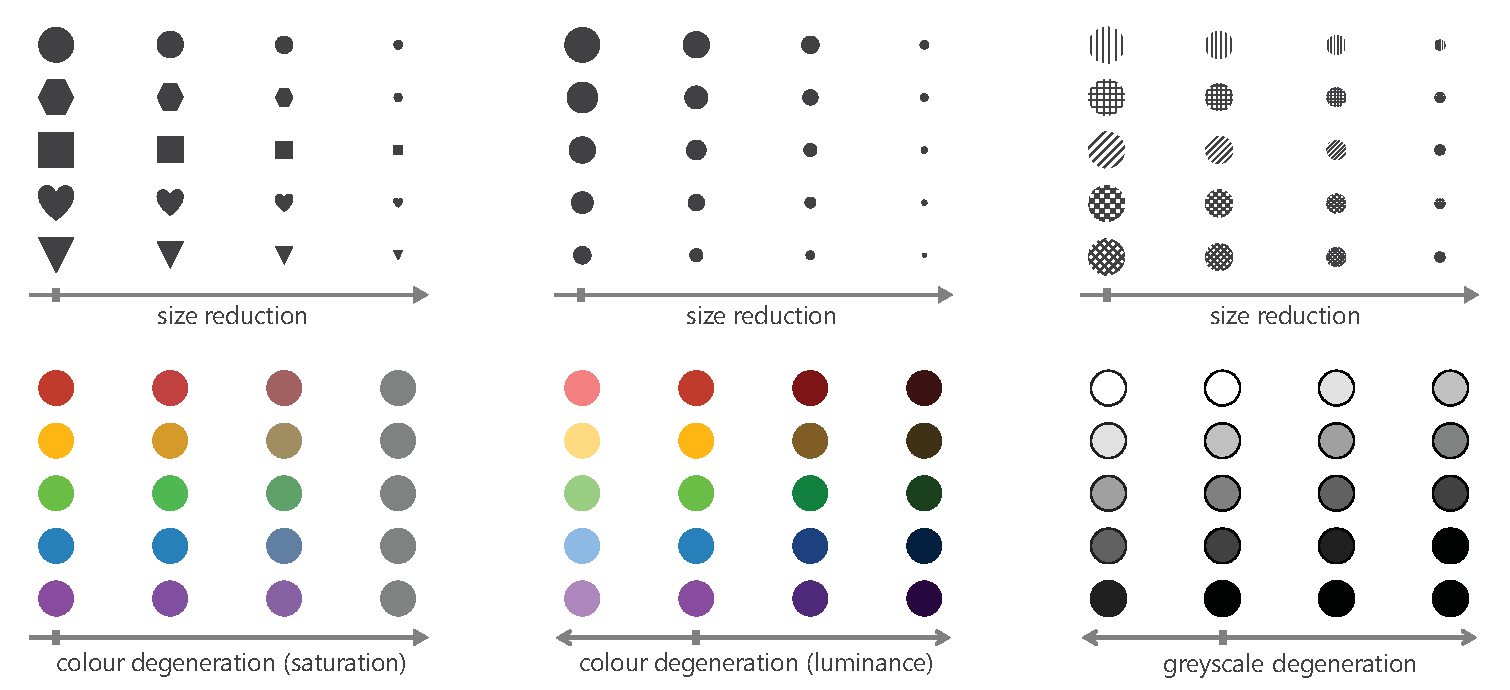
\includegraphics[width=0.95\textwidth]{images/filesystem/Unsafe}
\end{center}
\caption{Three different types of quality degeneration applied to several glyphs, each of which is encoded using a single retinal variable.
The original quality is indicated by a marker on the $x$-axis.
All variations of degeneration result in perception difficulties, however the effect is more so with size, saturation and luminance adjustments.}
\label{fig:reduction_degradation}
\end{figure*} 


\subsection{Background}
Perceptual guidelines discussed throughout this thesis can be adopted for more effective visualization. 
By using the correct data type to retinal variable mappings, prioritising dimensions based on their importance to tasks, and ensuring separability of dimensions, the glyph design process can be improved.

%This chapter extends on those foundations to provide a computation
Glyph designers will often use their creative intuition to ensure the diversity and legibility of different glyphs as is seen within the icon and font design communities.
Much of the work presented in this thesis so far has focused on the use of computation in combination with design principles to systematise the glyph design process in terms of what visual channels should be used and where. 
A further research question however would be \emph{``Is there a systematic approach to design a fail-safe glyph set?''}.

This work proposes a conceptual framework to optimise the design of a set of glyphs to provide a systematic way of ensuring fail-safe glyph encoding.
The framework is based on the \emph{Hamming} distance (Section \ref{sec:hamming}).
Due to the subjective nature of many design aspects, we introduce the concept of the \emph{quasi-Hamming distance} (QHD) (Section \ref{sec:qhd}).
Using this idea, we are able to transition from a qualitative assessment of perceptual distances in a design to a more quantifiable assessment based on this new metric.
For instance, when the minimal Hamming distance for a glyph set is one, the glyph set is vulnerable to ``noise'' during observation and exploration. 
If the minimal Hamming distance is two, the glyph set facilitates some error detection, whereby the viewer can use interaction (\eg, zooming-in, or looking at the legend) to investigate the error.
When the minimal Hamming distance is three or more, the glyph set facilitates some error correction at the receiving end.
This enables us to adjust the design to ensure a minimal Hamming distance among each glyph in a set of glyphs.
In addition to this novel concept for glyph design, this work makes the following additional contributions:  
%
\begin{itemize}
\vspace{-2mm}
\item
We outline several methods for estimating the QHD, and present two proof-of-concept of experiments for estimating the QHD based on manual grading by human participants, and through use of image-comparison metrics (Section \ref{sec:qhd}).
\vspace{-2mm}
\item
We present a case study on visualising file system events, where glyphs were designed to facilitate error detection and correction, and were evaluated by human participants and image-comparison metrics (Section \ref{sec:casestudy}).
\vspace{-2mm}
\item
We demonstrate the fail-safe file system event glyphs in a new visualization environment using event log data captured from Dropbox, a real-world distributed file sharing system \footnote{\url{www.dropbox.com}}.
\end{itemize}

\subsubsection{Hamming Distance}
\label{sec:hamming}

In information theory and data communication, a \emph{code} consists of a finite set of \emph{codewords}, each of which is a digital representation of a letter in an alphabet.
In the context of binary encoding, the \emph{Hamming distance}, proposed by Richard Hamming in 1950 \cite{Hamming:1950:Bell}, is a measure of the number of bit positions in which two codewords differ.
Considering all pairs of codewords in a code, the minimal distance is referred to as the minimal Hamming distance of the code.
In communication, there are two main strategies for dealing with errors that occur during transmission.
\emph{Automated error detection} allows the receiver to discover that any error has occurred and to request a retransmission accordingly.
\emph{Automated error correction} enables the receiver to detect an error and deduce what the intended transmission must have been.
Hamming defined the following principle:

\begin{figure}[h!]
\begin{center}
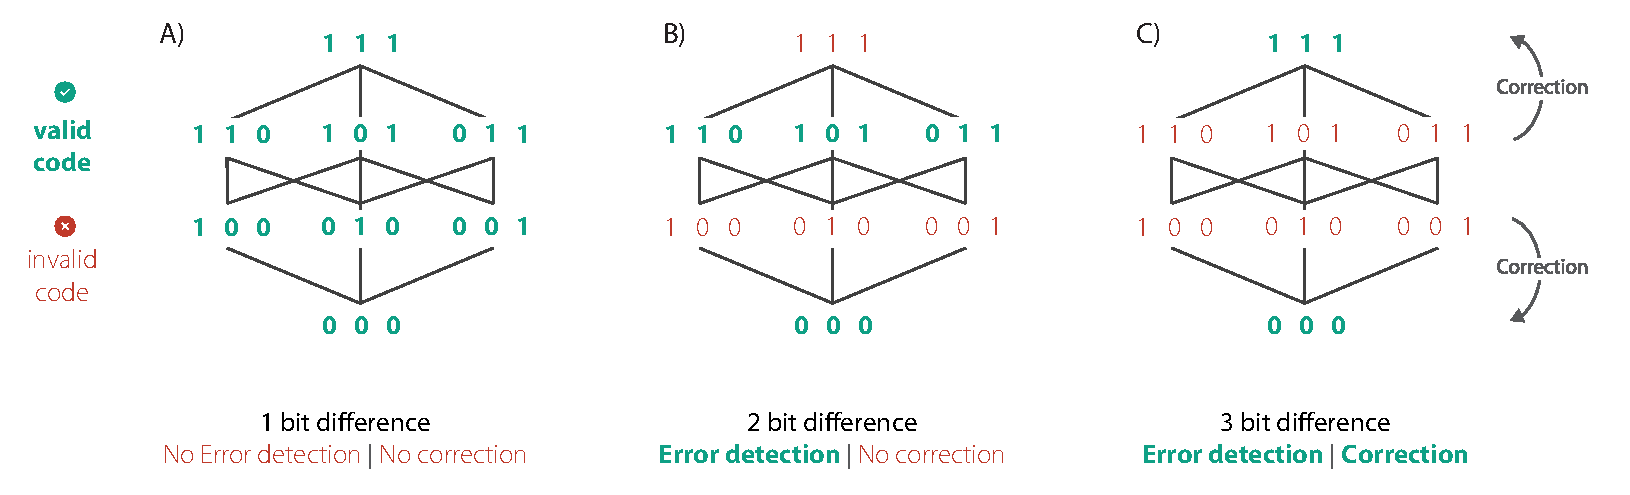
\includegraphics[width=\textwidth]{images/filesystem/latest/Hamming1}
\end{center}
\caption{Principles of error correcting codes.
A) A code with no error detection where every code is valid. No way of detecting errors and no way of correcting them.
B) A code with a distance of two bits between valid codes can detect errors but cannot correct since one change in any position will result in a valid code (knowing what changed is difficult).
C) A code with a distance of three bits between valid codes can detect errors and correct them.}
\label{fig:hamming}
\end{figure}

\noindent \textbf{Theorem.} A code of $d+1$ minimal Hamming distance can be used to detect $d$ bits of errors during transmission. A code of $2d+1$ minimal Hamming distance can be used to correct $d$ bits of errors during transmission~\cite{Hamming:1950:Bell}.

For example, given a three-bit code as illustrated in Figure~\ref{fig:hamming}, there are eight possible codewords.
One may select a subset of these codewords to construct a code with its minimal Hamming distance equal to two bits or three bits.
Figure~\ref{fig:hamming} B) shows such a code with four valid codewords and a minimal Hamming distance of two bits.
This code can detect one-bit errors since any change of a valid codeword by one bit would result in an invalid codeword, which would lead the receiver to discover the error.
Figure~\ref{fig:hamming} C) shows another code, with two valid codewords and a minimal Hamming distance of three bits.
This code can detect two-bit errors and correct one-bit errors.
When a valid codeword (\eg, 111) is changed by one bit during transmission (\eg, 110), the receiver can detect such an error and recover the intended codeword based on the nearest neighbour principle.
Of course, if a two-bit error occurred during transmission, the receiver would be able to detect the error but could not make a correct ``correction''.
Nevertheless, if it is known that two-bit errors are likely to occur then this should either be used as only an error detection code, or a code with a larger minimal Hamming distance should be used instead.

\subsubsection{A Quasi-Hamming Distance for Glyph Design}
\label{sec:qhd}

One can consider a set of glyphs as a code, and each glyph in the set is a valid codeword.
On presenting a glyph-based visualization to a user, there may be errors in the display and perception of a glyph.
If a viewer can detect that a perceived glyph is not quite ``right'', conscious or unconscious effort can be made to correct such an error.
Conscious effort, an analogy of error detection and repeated transmission, may typically include zooming in to have a close look, or consulting the legend.
Unconscious effort, an analogy of error correction, may include some Gestalt effects \cite{Chen:2014:CGF}, and inference from other visual information \cite{Rheingans:1995:PIV}.
Figure~\ref{fig:glyph_hamming} shows two example glyph sets, each with eight codewords.
Given the two display errors shown on the left, where an arrow glyph is skewed in a distorted printout, and a shape glyph is occluded by another shape.
Both errors can be detected, although the error for the arrow glyph will require more conscious effort to correct, although in this case that would be impossible due to the small distance between each glyph in the set. 
The star glyph can be corrected unconsciously due to Gestalt effects in combination with the greater distance between each of the glyphs.
These examples would suggest that it is possible to establish a conceptual framework, similar to the Hamming distance for error detection and error correction in glyph-based visualization.

\begin{figure}[t!]
\begin{center}
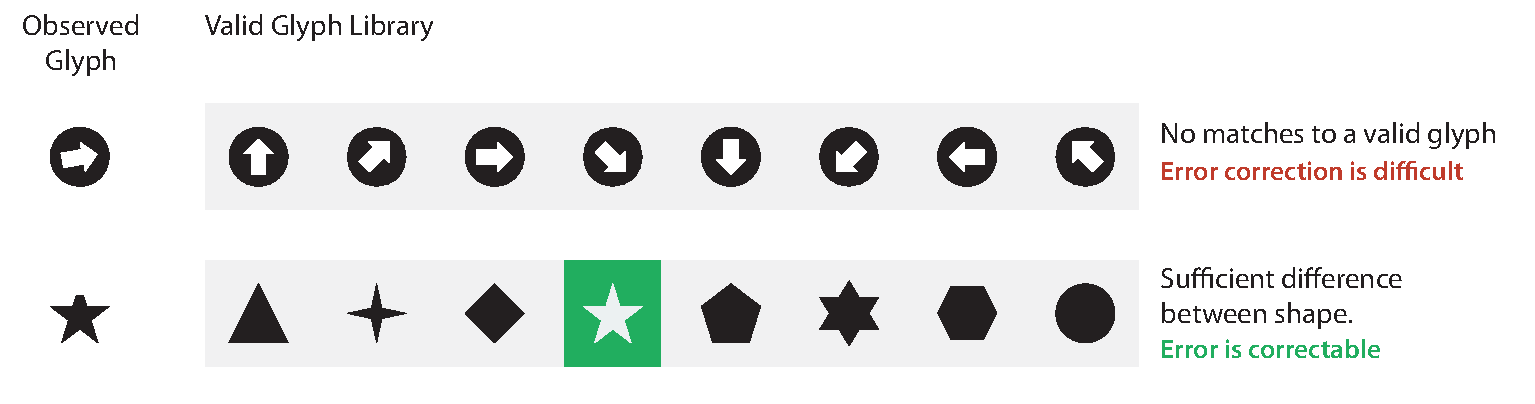
\includegraphics[width=\textwidth]{images/filesystem/latest/QHD}
\end{center}
\caption{Two examples that illustrate the phenomena of error detection and error correction in glyph-based visualization. (Above) A viewer may sense that the glyph on the left may not be correct in a distorted visualization, and consult the legend to correct the error. (Below) A viewer may unconsciously perceive the glyph on the left as a star shape due to Gestalt effects and apriori knowledge about the glyph set.}
\label{fig:glyph_hamming}
\end{figure}


Understandably, measuring the distances and errors in visual perception is not as simple as measuring those represented by binary codewords.
We propose an approximated conceptual framework based on the principle of Hamming distance, which we call a \emph{Quasi-Hamming Distance} (QHD).
The term ``quasi'' is used to show that the distance measure is an approximate, and that the quantitative measure of perceptual error is also approximated.
Therefore, the main research questions are:
i) can we establish a measurement unit common to both measures?; and
ii) given a glyph set, how can we measure the distance between those glyphs?\\

\noindent\textbf{Can we establish a measurement unit common to both measures?} A ``bit'' can be used as the common unit for both distance and error measurement.
Consider an ordered retinal variable, such as brightness or length, as a code $C$.
Theoretically, $C$ can have a set of codewords $\{ c_1, c_2, \ldots c_n \}$ such that the difference between two consecutive codewords is the just-noticeable difference (JND) of this retinal variable.
We can define the QHD between each pair of codewords $c_i$ and $c_j$ as $|i-j|$ bits.
During display and visualization, if $c_i$ is mistaken for $c_j$, we can call this a $d$-bit error where $d=|i-j|$.
Now let us extend this concept to a less ordered retinal variable (\eg, colour hue).
Theoretically, we can construct a code $C$ by uniformly sampling the space of the retinal variable (\eg, the CIE L*a*b* colour space) while ensuring that every pair of samples differ by at least the JND of this channel.
These codewords can be organised into a network, where the distance between any two codewords can be approximated proportionally according to the JND (\emph{i.e.}, JND = 1 bit).
The possible perception error rate with a code that maximises the number of codewords based on JND is likely to be very high.
In practice, a glyph set is designed using a small subset of visual channels.
However, it is more common to use several visual channels in the multivariate.
Therefore a QHD measure based on JND would be too fine to use in practice, although JND can provide an \emph{absolute reference measure} once measures for the visual channels used in visualizations have been obtained.\\

\noindent\textbf{Given a glyph set, how can we measure the distance between glyphs?} One may consider using the following methods:
\begin{enumerate}
\vspace{-1mm}
\item \textbf{Estimation by expert designers.} This practice has existed in design exercises such as the development of traffic signage (discussed in Chapter \ref{chap:related_work}, Section \ref{sec:relwork_glyphs}) and icons in user interfaces.
To formalise this practice, designers can explicitly estimate and label the distance between each pair of glyphs in a glyph set.
While this approach may be most convenient to the designers, its effectiveness depends very much on the experience of the designers concerned and it is easy to overlook certain types of display and perception errors;
\vspace{-1mm}
\item \textbf{Crush tests.} This test was introduced in Chapter \ref{chap:glyph-tax} to simulate how changes in size affect the perception of glyph features.
By simulating the various causes of perception error, such as those illustrated in Figure~\ref{fig:reduction_degradation}, we can determine the level at which glyphs become indistinguishable.
The corresponding level of degeneration can be defined as a QHD.
While this approach would yield more consistent estimation of a QHD, more research would be required to compile a list of different causes of errors and define coherent levels of degeneration across different causal relationships;
\vspace{-1mm}
\item \textbf{Task-based evaluation.} Similar to (2), one can simulate different visualization conditions, enlist users to perform their tasks, measure their performance, and transform performance measures to a QHD.
On one hand, this approach is perhaps most semantically meaningful for a particular glyph set in a specific application context.
On the other hand, the performance measures collected may feature many confounding effects, while there may only be a small number of users available for such an evaluation;
\vspace{-1mm}
\item \textbf{User-centric estimation.} One may conduct a survey among human participants about how easy or difficult it is to differentiate different glyphs. By removing task-dependency in (3), more participants can be involved in such a survey, yielding a more reliable estimation of the QHD.
Recent efforts have taken place to crowd source distances between simple shapes, colours, and sizes to create what are called \emph{Perceptual Kernels} \cite{demiralplearning}; and
\vspace{-2mm}
\item \textbf{Computer-based similarity measures.} A large collection of image similarity measures exist in the literature~\cite{Sahasrabudhe99, Eler08}.
%It is likely that we will be able to find measures that are statistically close to a user-centric estimation in the long term.
However, there are few metrics available that are designed for measuring the glyph similarity.
A good long term approach would be finding metrics that are statistically close to a user-centric estimation.
\end{enumerate}

To demonstrate the feasibility of estimating a QHD, we conducted two proof-of-concept experiments based on methods (4) and (5).
We conducted a survey among twenty participants, all of whom are either employees or students at University of Oxford.
About 50\% encountered glyph-based visualization in their course or work.
After a brief introduction, the participants were asked to rate how difficult or easy it was to differentiate 104 pairs of glyphs using an integer scale from 0 to 10.
The survey was conducted during an informal lunch, where pizzas were served.
No cash payment was involved.
The results of one participant were considered an outlier and were not included in the statistics.

\begin{figure*}[t!]
\begin{center}
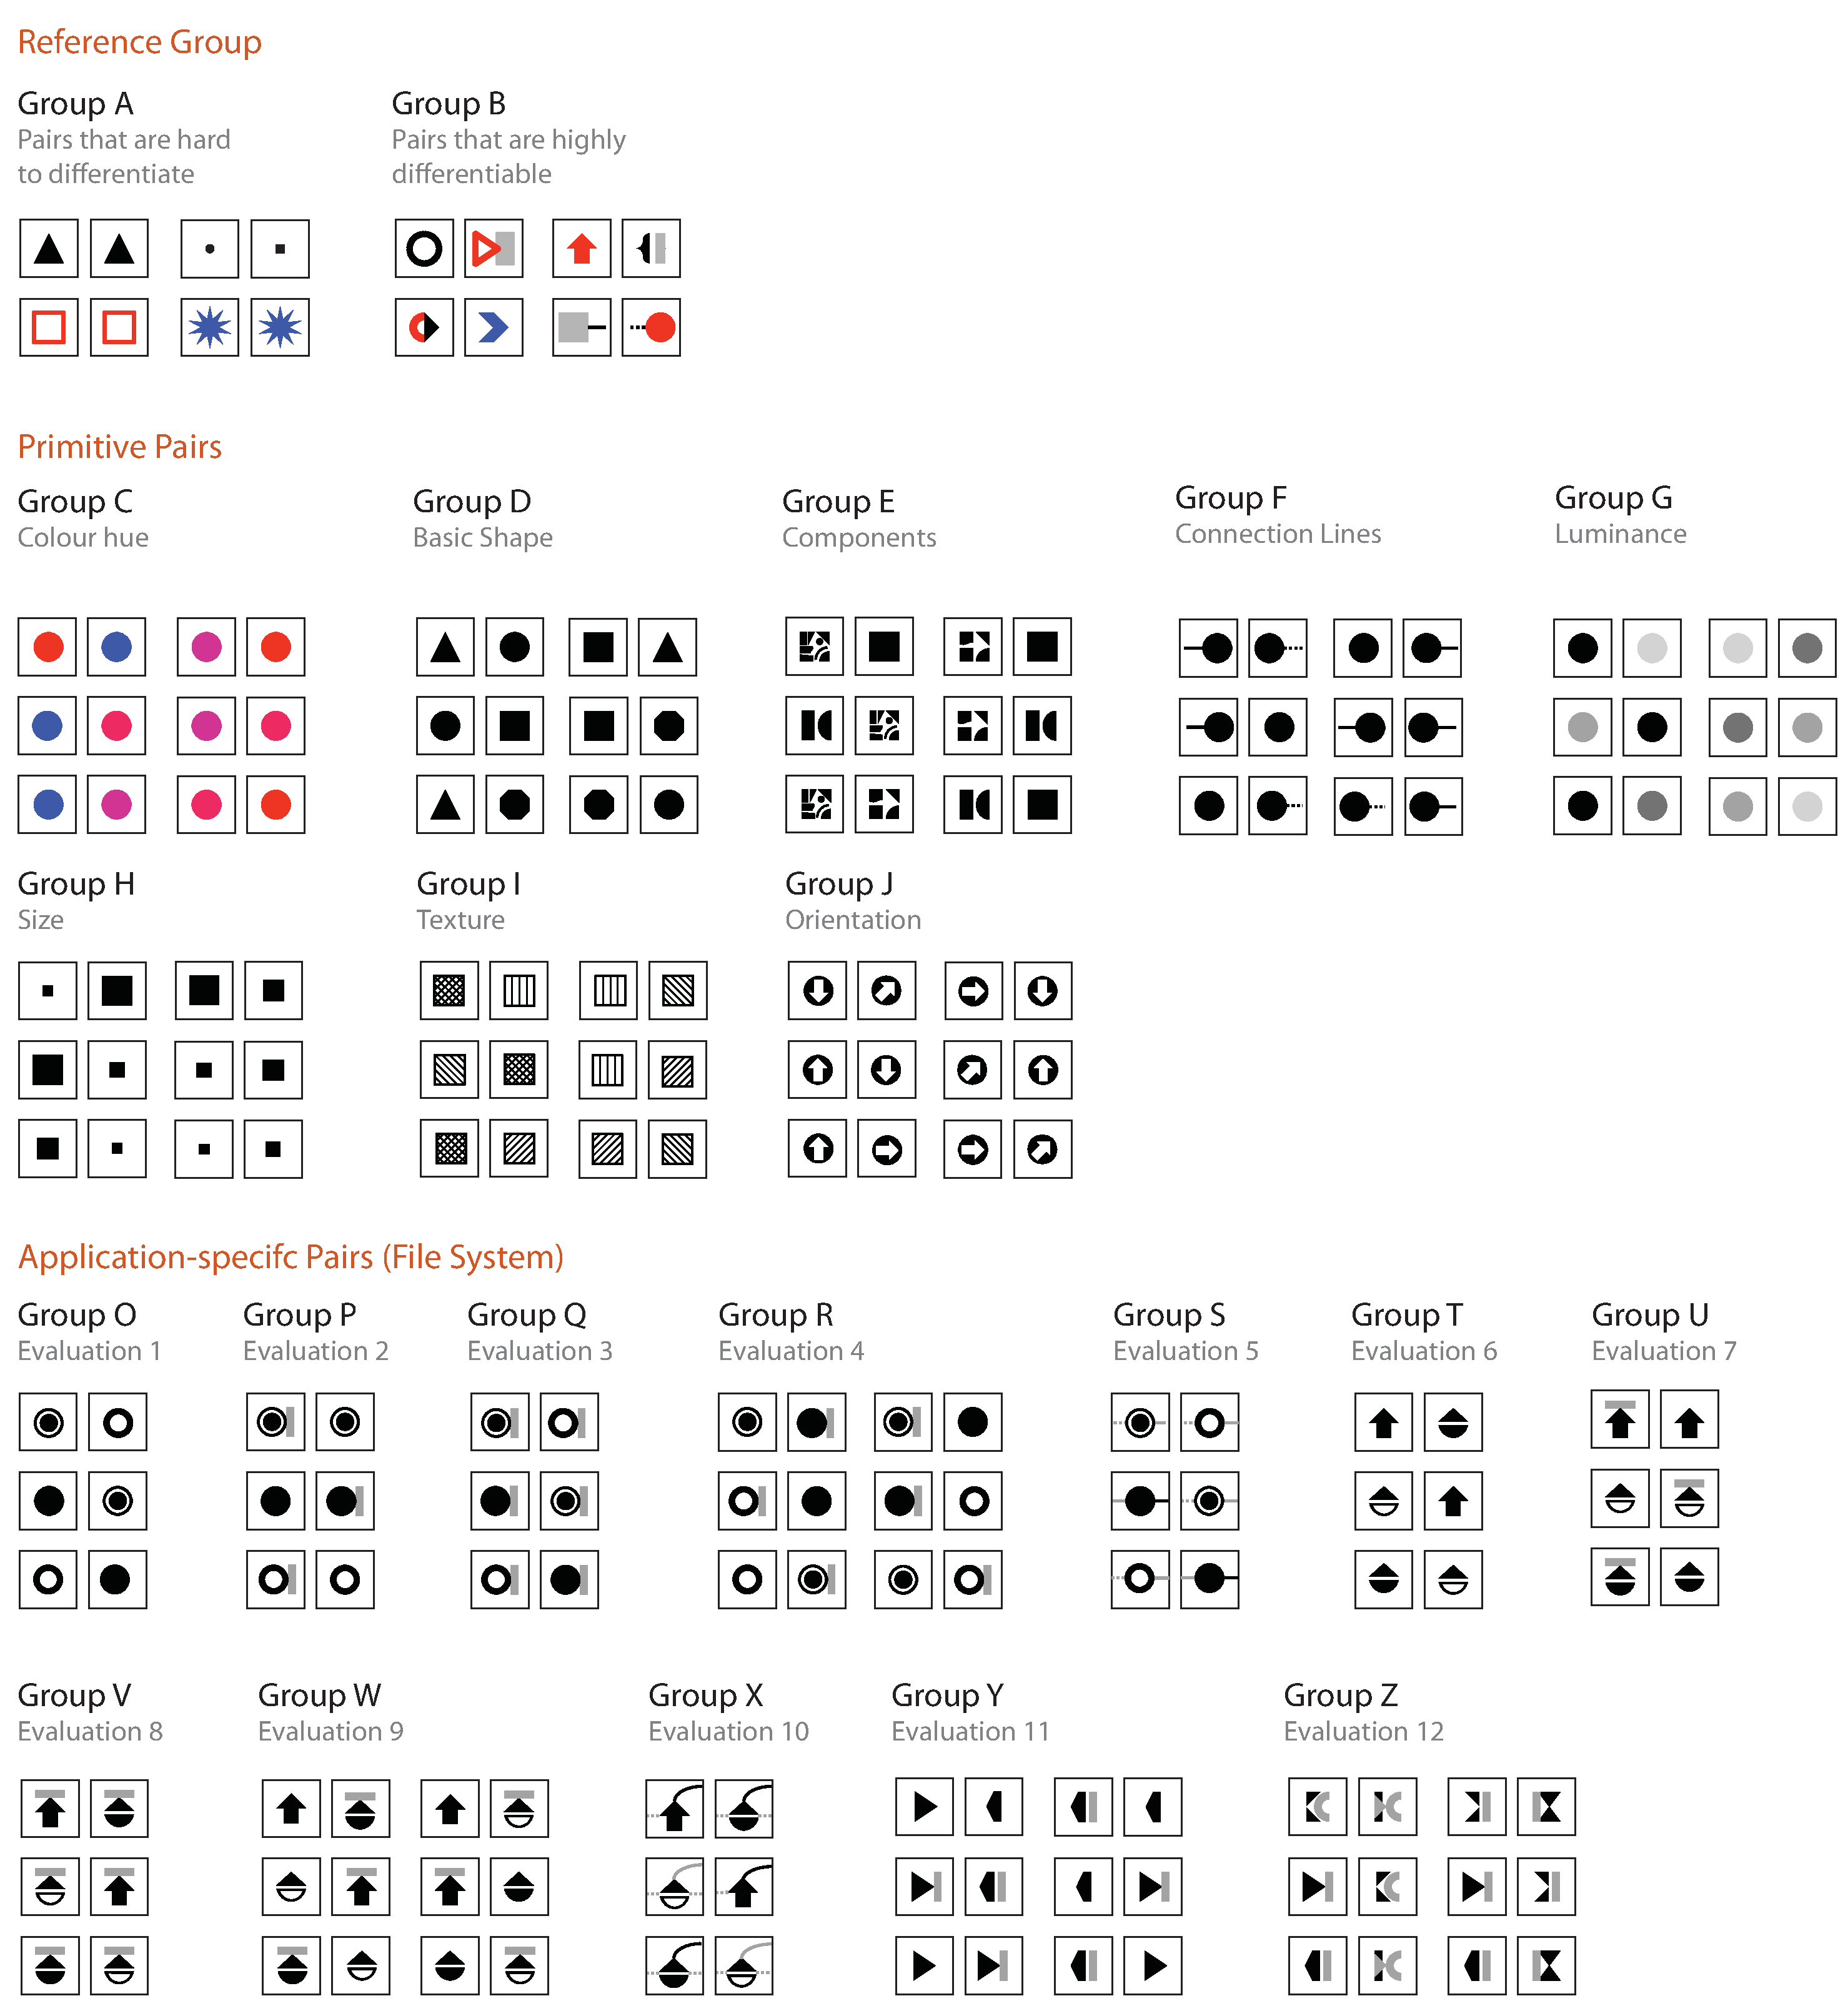
\includegraphics[width=\textwidth]{images/filesystem/evaluation_groups}
\end{center}
\caption{104 stimulation pairs are split in to three groups representing: the reference group; primitive pairs; and application-specific pairs.}
\label{fig:evaluation_groups}
\end{figure*}


Illustrated in Figure \ref{fig:evaluation_groups} are the 104 stimuli pairs divided into three categories: eight \emph{reference pairs}; forty-eight \emph{primitive pairs}; and forty-eight \emph{application-specific pairs}.
We will discuss the last category in detail in Section \ref{sec:application}.
The ninety-six primitive and application-specific pairs were mixed together in a randomised order.
The eight reference pairs were placed at positions 1, 2, 35, 36, 69, 70, 103, and 104 to help participants regularise their scores and to enable a temporal consistency check.

The reference pairs are divided into two groups.
Group A consists of four pairs of very similar glyphs, and Group B consists of four pairs of very different glyphs. 
We expected that participants would assign very low scores (difficult to differentiate) to those in A and high scores (easy to differentiate) to those in B respectively.
We placed one pair from A and one from B at regular intervals.
The average scores for the four pairs in group A are (0.0, 0.4, 1.4 and 2.8) respectively and those for group B are (9.3, 9.0, 8.9, 9.7) respectively, indicating that statistically, they have served as references for the minimal and maximum QHD in this survey.

The primitive pairs consist of eight groups for estimating the QHD in relation to eight visual channels, namely colour hue, shape, components, connection lines, luminance, size, texture, and orientation.
Each group has six pairs of stimuli, facilitating pairwise comparison of four different codewords for each channel.
For hue and luminance channels, after choosing the first and fourth codewords, we used a perceptually uniform colour model (Hunter's Lab) \cite{hunter1958photoelectric} to determine the second and third codewords at 50\% and 75\% distance from the first.
The upper part of Figure~\ref{fig:eval_glyph_scores} E shows a small selection of survey results, where we converted the $[0, 10]$ score range to a $[0, 5]$ QHD range.
We considered any QHD $<2$ as potentially risky for error detection, and any QHD $<3$ as potentially risky for error correction.

\begin{figure*}[t!]
\begin{center}
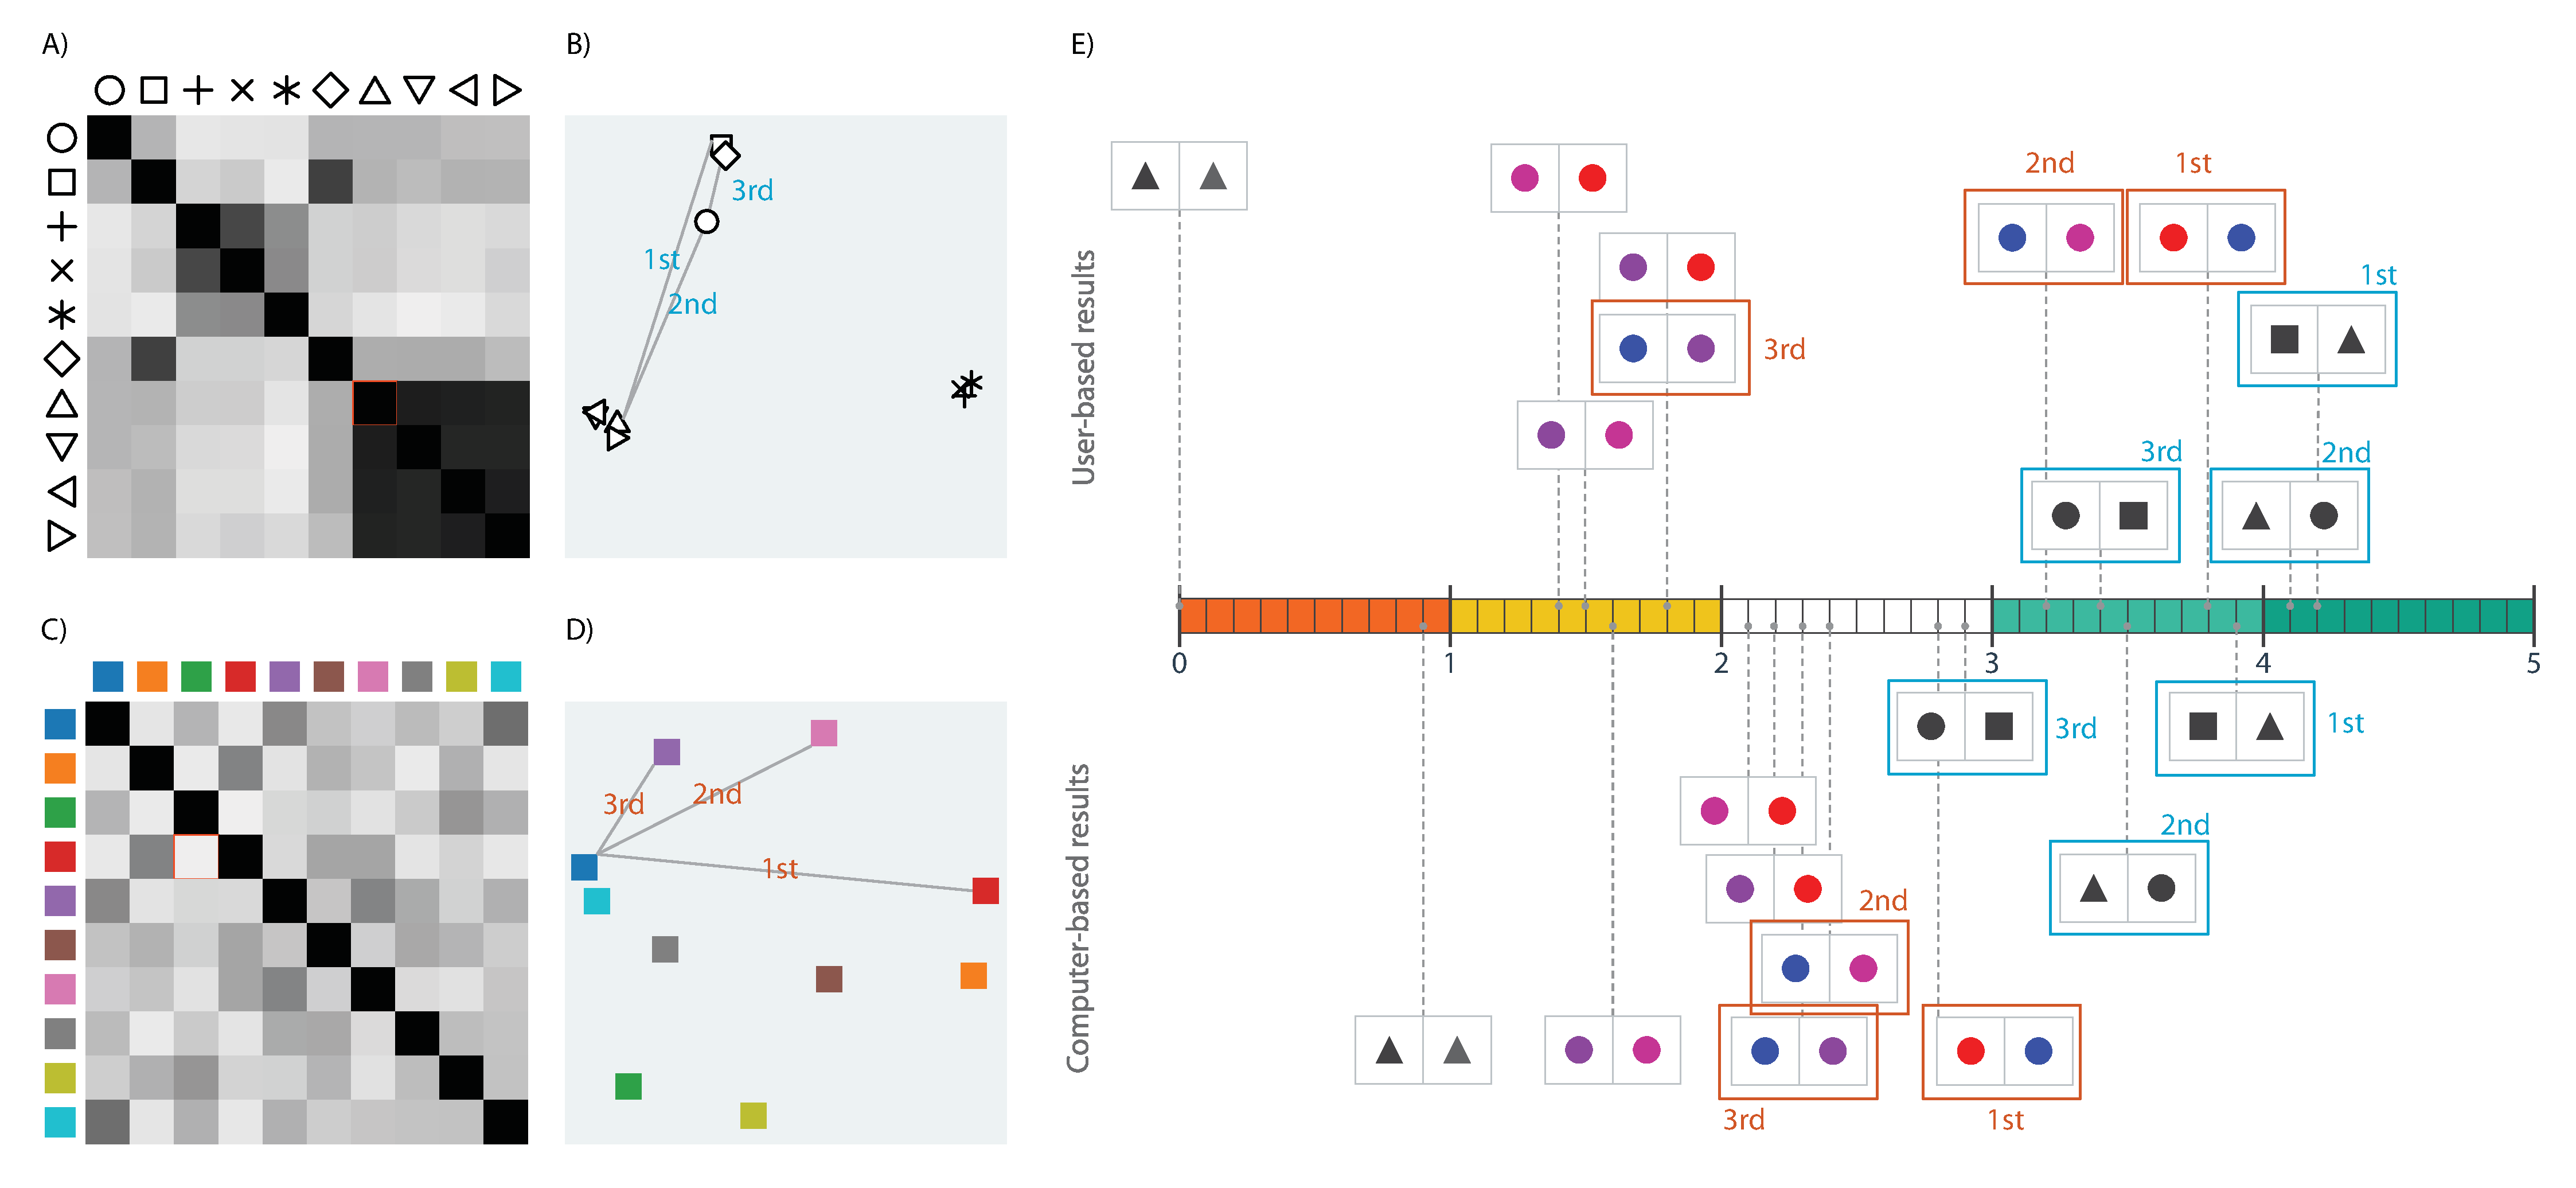
\includegraphics[width=\textwidth]{images/filesystem/perceptual_kernal_validation}
\end{center}
\caption{Reproduced figures from work by Demiralp \etal \cite{demiralplearning} (A-D) with respect to results from analyses in this work (E).
A) Distances between colours shown as a heat map.
The higher the similarity, the darker the square.
B) Shapes arranged in 2D space by their similarity. This is calculated using multidimensional scaling (MDS) of the perceptual kernel.
C) Distances between colours shown as a heat map.
D) Colours arranged in 2D by their similarity (again created from MDS of their perceptual kernel).
E) Results from our user-based and computation-based analyses.
The results are correlated with results from \cite{demiralplearning}.
The top three perceptually distant shapes and colours are marked across the results.}
\label{fig:eval_glyph_scores}
\end{figure*}

In our second experiment, we measured the similarity between each pair of glyphs using a computer-based metric.
This metric combines differences in pixel colour with spatial occupancy.
The former captures a variety of feature differences such as colour, luminance, size, and orientation.
The difference is defined as the mean Euclidean distance between all corresponding pixels in the two images representing the pair of glyphs.
The latter captures some location-invariant features such as spatial occupancy, and is defined as the difference between the numbers of pixels with $\leq 80\%$ luminance.

Both difference measures are first normalised to the $[0, 1]$ range, and are then scaled to the QHD range from the user-centric survey, before being combined into a single metric.
The lower part of Figure~\ref{fig:eval_glyph_scores} E shows the computed similarity measures for the same selection of stimuli pairs.

\subsection{File System Event Visualization}
\label{sec:casestudy}

The problem of visualizing file systems plays a significant role in the short history of computer-assisted visualization.
In 1991, Johnson and Shneiderman, who were motived by the need to visualise the structure of a file system, published their seminal paper on treemaps~\cite{johnson91}.
Today, not only are file systems larger, they are also shared by many more users.
One important aspect of a file system is to support collaborative activities, such as sharing files within multi-partner projects, or developing software with a team geographically distributed programmers.
While there are text-based mechanisms for recording events in relation to a file system or a specific folder, the amount of data contained in typical log files can easily escalate to the point where it becomes too overwhelming for anyone to read.
To our knowledge, there is no effective visualization technique for allowing users of such collaborative environments to observe events in a cost-effective manner.

In this case study, we designed and developed a novel glyph-based visualization tool for observing events in a file system.
There are several technical challenges.
Firstly, the hierarchical nature of the file system needs to be depicted so that the spatial context of where a particular event has occurred can be identified.
Secondly, the temporal information about events needs to be conveyed so that the activity ordering can also be observed and reasoned.
Thirdly, there are a wide range of activities (\eg, copying a file, modifying a file) that are typically performed, which would need to be distinguishable in a visualization.
Finally, the visualization should be able to support collaborative environments by depicting activities by a number of users.

\begin{figure*}[t!]
\begin{center}
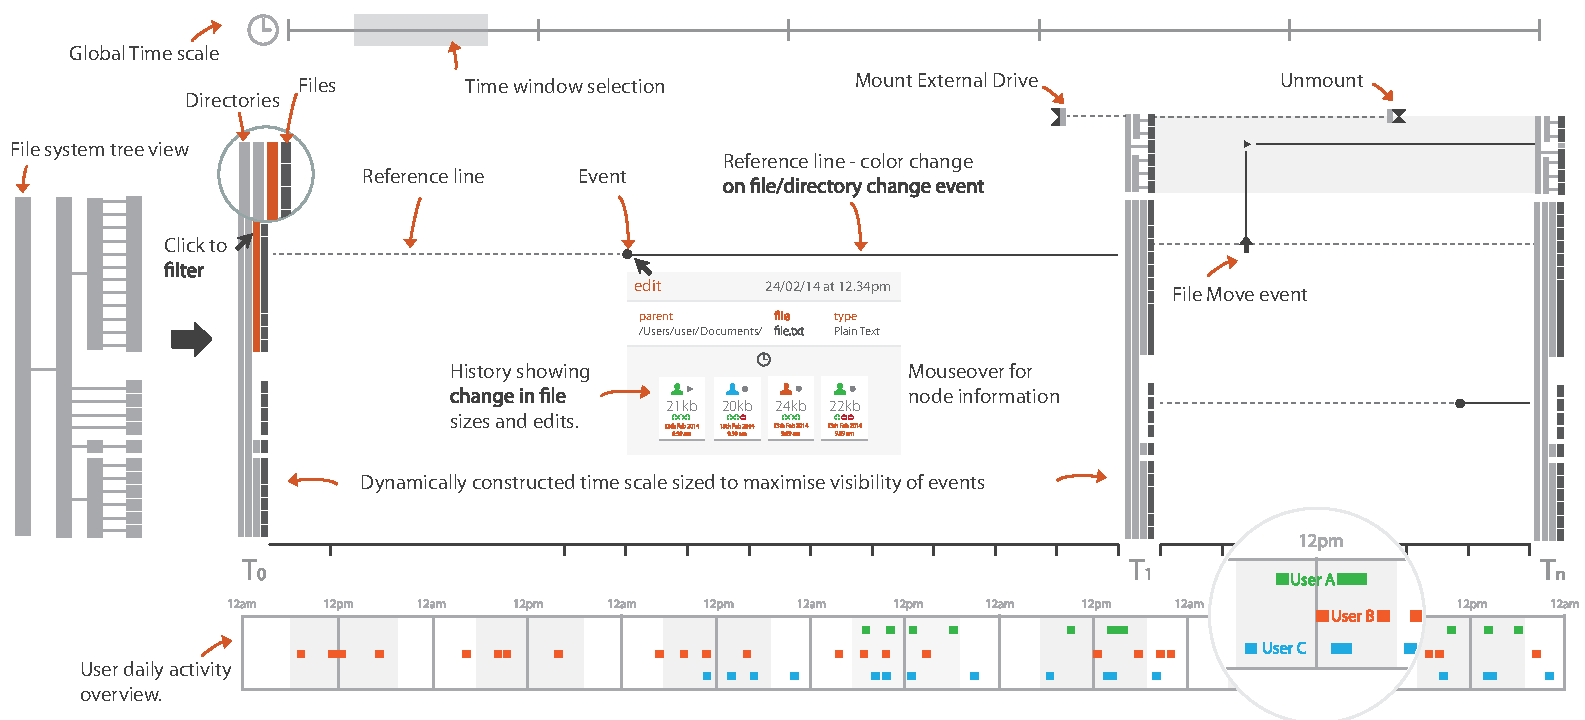
\includegraphics[width=\textwidth]{images/filesystem/system_overview}
\end{center}
\caption{We use a timeline approach with a condensed file system hierarchy at the left of the visualization.
File system activities are depicted by glyphs on the timeline, with connecting lines to show their place in the file system.
Keyframes are displayed to depict significant changes to the file system hierarchy, or at user-specified time intervals.
Interaction with the mouse displays a context aware box, with detailed information on the selected file, directory, and activity.}
\label{fig:system}
\end{figure*}

Figure~\ref{fig:system} presents an overview of the adopted visualization design.
The visualization consists of a number of different components:
\begin{enumerate}
\item \textbf{Central Panel}. The main activity window where events performed on the file system are displayed on a timeline using glyphs. 
To the far left is the file system tree view, which represents the file system using a traditional tree representation where directories are shown as light grey nodes and files shown as dark grey nodes.
Since most directories are likely to contain files, leaf nodes are typically file objects.
This tree is shown as a condensed display to the left of the main timeline and serves as a reference to the spatial context of the file location.
File system events are positioned corresponding to the file system hierarchy.
Connected lines are displayed relating file activities back to a position in the file system hierarchy.
For events that involve a change in the file system hierarchy, such as copying or moving files, these connecting lines also indicate the new position of the file.
The condensed file hierarchy also serves as a ``keyframe'', where the current state of the file system hierarchy is shown, either after a significant change to the hierarchy (\eg, copying files, or mounting an external drive), or at a particular time interval specified by the user.
Finally, the file hierarchy can also be used to select the directory of interest that should be shown on the visualization.
This provides a mechanism for ``zooming in'' to a particular directory, or ``zooming out'' to view the root directory;

\item \textbf{Top Panel}. At the top of the display is a temporal filter; allows queries for a desired time period to be displayed in the \emph{central panel};

\item \textbf{Bottom Panel}. A daily activity overview: provides a temporal summary of user activity.
\end{enumerate}

The interface also supports detail on demand via a pop-up window for every file system event. 

\subsubsection{Design Process}

The concept of the QHD has been considered throughout the design, development, evaluation, and application of the glyph-based file system visualization tool.
Figure~\ref{table:fileoperations} shows eighteen glyphs for the most common events in file systems.
These events include creation, modification, deletion, copying, moving, and renaming.
These actions may be applied to a file, directory, device, shortcut (symbolic link), or meta-data.
The design of these event glyphs evolved through several stages:

\begin{enumerate}
\item\textbf{Initial Design.} We first designed a set of glyphs that were heavily influenced by the need for metaphor (see the \emph{natural mappings} design guideline in Chapter \ref{chap:strategies}).
The glyphs were placed in context with the overall visual design of the visualization tool as shown in Figure~\ref{fig:system}.
This presented an opportunity to appreciate how these glyphs may be used, and how glyph size for instance would affect the visual channels that could be used.
Here, we decided that the basic glyph design should not feature colour hue. 
This powerful visual channel should be reserved to show different users or to colour-code files or directories for example.

\item\textbf{Expert Estimation.} Four visualization researchers took part in this work, and all have publications in the area of glyph-based visualization.
Using knowledge from Chapter \ref{chap:related_work} focused on visual channels and their properties, and design guidelines from Chapter \ref{chap:strategies}, combined with our experience in glyph design, the original designs were improved.
We noticed that although we could reach agreement as to how easy or difficult it can be to differentiate pairs of glyphs, we could not easily agree on the reasons why.
When we explicitly tried to determine the QHD between a pair of glyphs, we were often influenced by many different features including component shapes, convexity, aspect ratio, and curvature for example.
This experience led us to appreciate the complexities involved in estimating the QHD.
Many of the glyph designs in Figure~\ref{table:fileoperations} stabilised at this stage. 

\item\textbf{Crush Tests.} We applied crush tests first used in Chapter \ref{chap:glyph-tax} to all glyphs designed during the case study.
This test was used to determine if the global features of each glyph were distinguishable at even low resolutions.
In several cases, we carried out systematic tests by applying consistent zoom factors to all glyphs.
Moreover, when considering individual glyphs, we carried out \emph{ad hoc} crush tests by using facilities in our drawing software, such as zooming, and overlaying a translucent shape on top of glyphs.

\item\textbf{Human-centric Estimation.} We conducted a survey to gain a better understanding about the QHD in the context of individual visual channels (see Section~\ref{sec:qhd}), and to evaluate our event glyphs in Figure~\ref{table:fileoperations}.
We considered twenty different glyph designs, for which there would be one hundred and ninety pairwise comparisons.
We selected forty-eight pairs that were considered potentially more risky than other pairs.
We found that only one pair scored below two bits in terms of QHD in the survey.
The final glyph designs did not include this pair.
The details of this evaluation will be given in Section \ref{sec:eval_glyphs}.

\item\textbf{Computer-based Similarity Measures.} We used the same metric as mentioned in Section~\ref{sec:qhd} to measure the QHD of the forty-eight pairs that might be a risk.
We found that they all passed this QHD test.
The details of this evaluation will be also given in Section~\ref{sec:eval_glyphs}.

\item\textbf{Deployment in Software.} In addition to the above design efforts based on the concept of a QHD, we incorporated the glyph set into the visualization tool and used the tool to visualise events in a Dropbox folder and a Git repository.
This made it possible to gain direct insight into how these glyphs might be viewed and interpreted in practical applications.
The details of this deployment will be discussed in Section~\ref{sec:application}.
\end{enumerate}

\begin{figure*}[t!]
\begin{center}
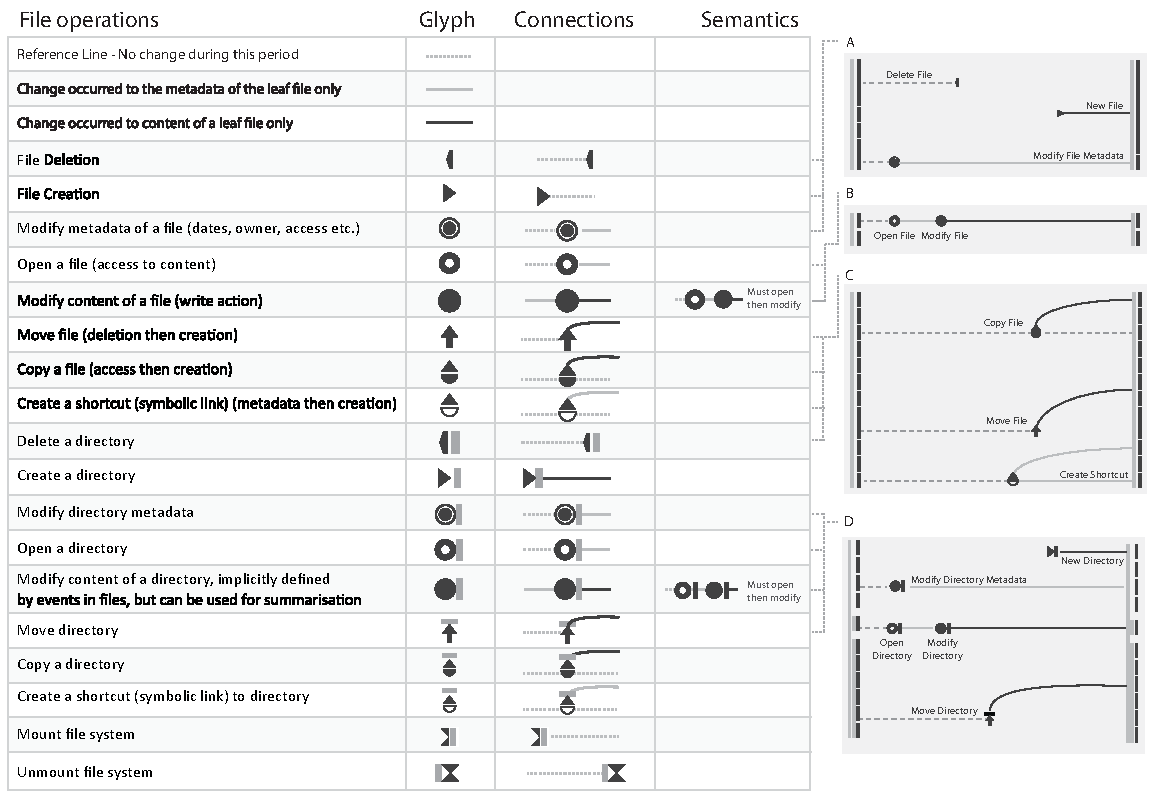
\includegraphics[width=0.99\textwidth]{images/filesystem/table_new}
\end{center}
\caption{Eighteen glyphs designed to represent different events in file systems.
Each event is associated with its primary glyph representation in the second column.
In addition, an event may be associated with special signatures in terms of connection (in the third column) and semantic ordering (in the fourth column).
Semantic ordering refers to how some glyphs will only ever appear in conjunction with another glyph (\eg, modifying a file requires first opening the file \emph{then} modifying its contents).}
\label{table:fileoperations}
\end{figure*}

Differentiability is only one aspect of glyph design.
We have to consider other aspects such as how easy it is to learn and remember glyphs, how glyphs may be connected, and how they may be ordered if the corresponding events happened to the same file or directory?
As shown in Figure~\ref{table:fileoperations}, we utilised similar designs for files and directories to facilitate learning and memorisation.
We also considered how they may be connected.
The three types of connection lines as shown at the top of the Figure~\ref{table:fileoperations} and their different positions (shown in the third column), may add additional features to help differentiate glyphs.
For example, all lines connecting to a \emph{deletion} glyph will always come from the left, and all connecting to a \emph{creation} glyph will extend to the right.
All lines connecting a \emph{copy} or \emph{move} glyph will suggest a spatial shift vertically.
Additionally, semantic ordering, such as \emph{open} before \emph{read}, can make the difference in increasing the QHD of the glyph designs as illustrated on the right side of Figure~\ref{table:fileoperations}.

\subsubsection{Evaluation}
\label{sec:eval_glyphs}

We evaluated those glyphs in Figure~\ref{table:fileoperations} based on the QHD obtained from a human-centric survey and by using computer-based similarity measures.
We used the same survey and metrics as described in Section~\ref{sec:qhd} since this allowed for comparison of the QHD for our glyph set against that of the reference pairs and primitives discussed in Section~\ref{sec:qhd}.
%Note that for our glyphs only the potentially risky pairs were evaluated.

\begin{figure*}[b!]
\begin{center}
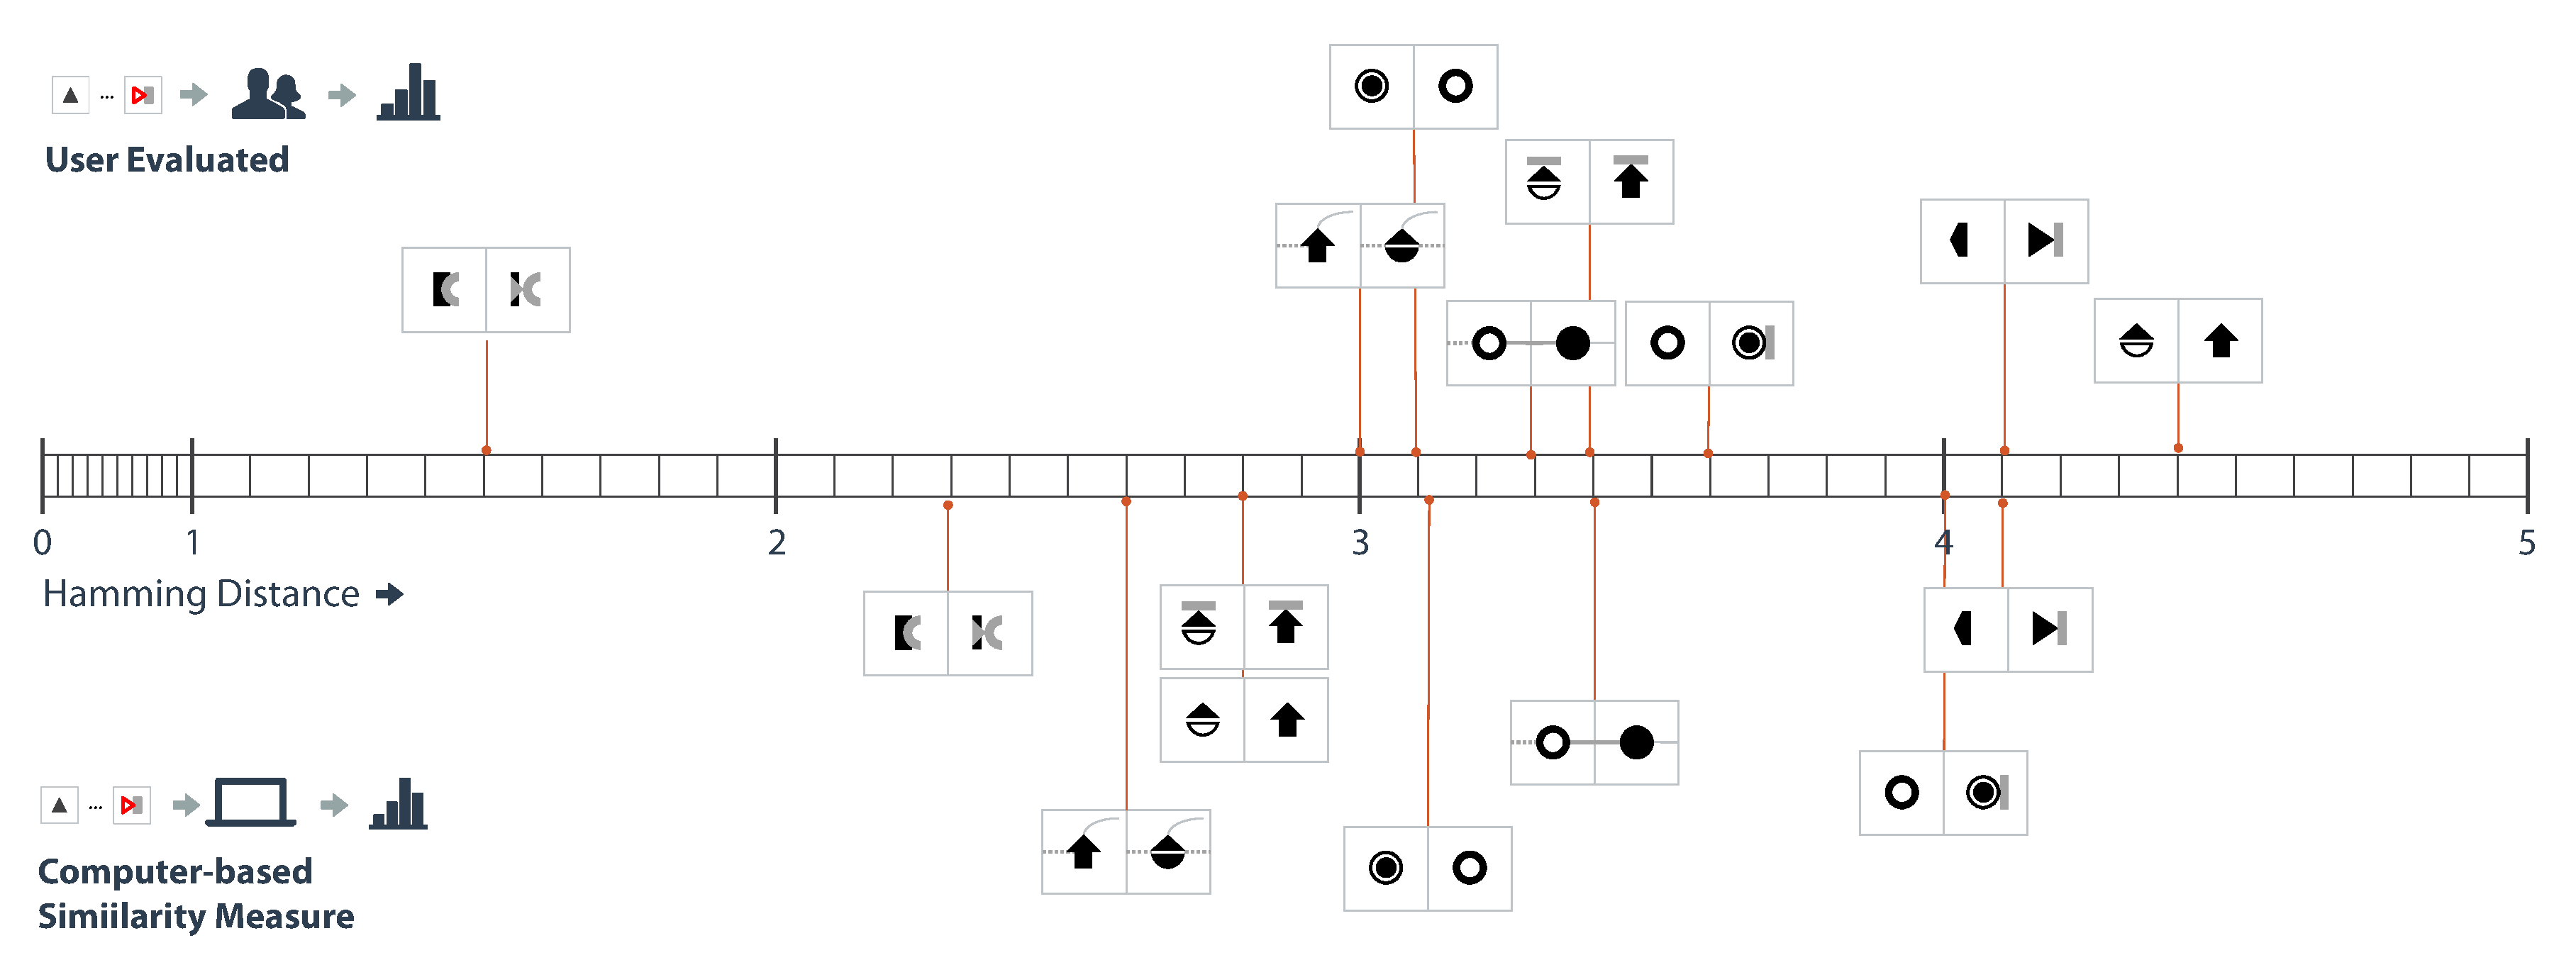
\includegraphics[width=\textwidth]{images/filesystem/Comparison_ourglyphs}
\end{center}
\caption{Sample of results for the file visualization glyph pairs used in both the user-centric estimation (top) and by computer-based similarity measure (bottom).
Low values indicate difficult to differentiate glyphs (bar colour coded in orange/yellow), whilst high values indicate easy to differentiate glyphs (bar colour coded in greens).}
\label{fig:our_glyph_scores}
\end{figure*}


The human-centric estimation provided us with most meaningful insights about the quality of the glyphs.
The 104 pairs of glyphs evaluated by participants have an average QHD of 2.9 bits.
Figure \ref{fig:evaluation_groups} shows the 22 comparison groups used in this evaluation. 
The average QHD for the reference pairs (Groups A and B) is 2.7 bits.
The average for the primitive pairs (Groups C, D, E, F, G, H, I, J) is 2.6 bits.
The average for the potentially risky pairs in our file system glyph set (Groups O, P, Q, R, S, T, U, V, W, X, Y, Z) is 3.2 bits.
Almost all of our glyph pairs have their QHD above 2 bits, except one pair (QHD = 1.5 bits) which was not used in the final design.
The upper part of Figure~\ref{fig:our_glyph_scores} shows a selection of the survey results.

Meanwhile, the computer-based metric also measured our glyph pairs favourably.
The average QHD estimated by the metric is normalised to have the same min, mean and max as the human-centric estimation.
The complete set of 104 glyph pairs have an average QHD of 2.9 bits
The average QHD for the reference pairs is 2.6 bits.
The average for the primitive pairs is 2.7 bits.
The average for the potentially risky pairs in our glyph set is 3.1 bits.
The lowest QHD for our potentially risks glyph pairs is 2.1 bits.


Subsequent research presented by Demiralp \etal in their work on Perceptual Kernels\cite{demiralplearning} further validated our user-based and computer-based results.
Their findings for shape and colour distances are shown in Figure \ref{fig:eval_glyph_scores} A - D.
These results are shown to be consistent with the overall results extrapolated from the user- and computer-based metrics in Figure \ref{fig:eval_glyph_scores} E. 

The evaluation also showed some interesting phenomena.
The additional features added to the directory glyphs have reduced the QHD among directory glyphs.
For example, when comparing Group O and Group Q, where the glyphs for \emph{creation}, \emph{modify metadata}, and \emph{modify content} were compared within the context of files and directories respectively, human-centric estimation shows a noticeable difference.
The average QHD for Group O (files) is 3.4 bits and that for Group Q (directories) is 2.6 bits.
Similarly, for Group T and Group V where \emph{move}, \emph{copy}, and \emph{short cut} glyphs were compared, the average QHD for Group T (files) is 3.3 bits, and that for Group V (directories) is 2.8 bits.
The computer-based similarity measures suggest little difference between O and Q and between T and V.
This indicates a need for further research to better understand the role of integral and separable visual channels.

\subsubsection{Application}
\label{sec:application}

To demonstrate the applicability of the above glyph encoding scheme, we developed an interactive visualization tool for visualising event log data.
In addition to the glyph-based visualization, the system supports a variety of interactions including: file system event filters; user filters; file system navigation; temporal filters; and details on demand;
Here we discuss a use case with Dropbox logs.

\begin{figure*}[ht!]
\begin{center}
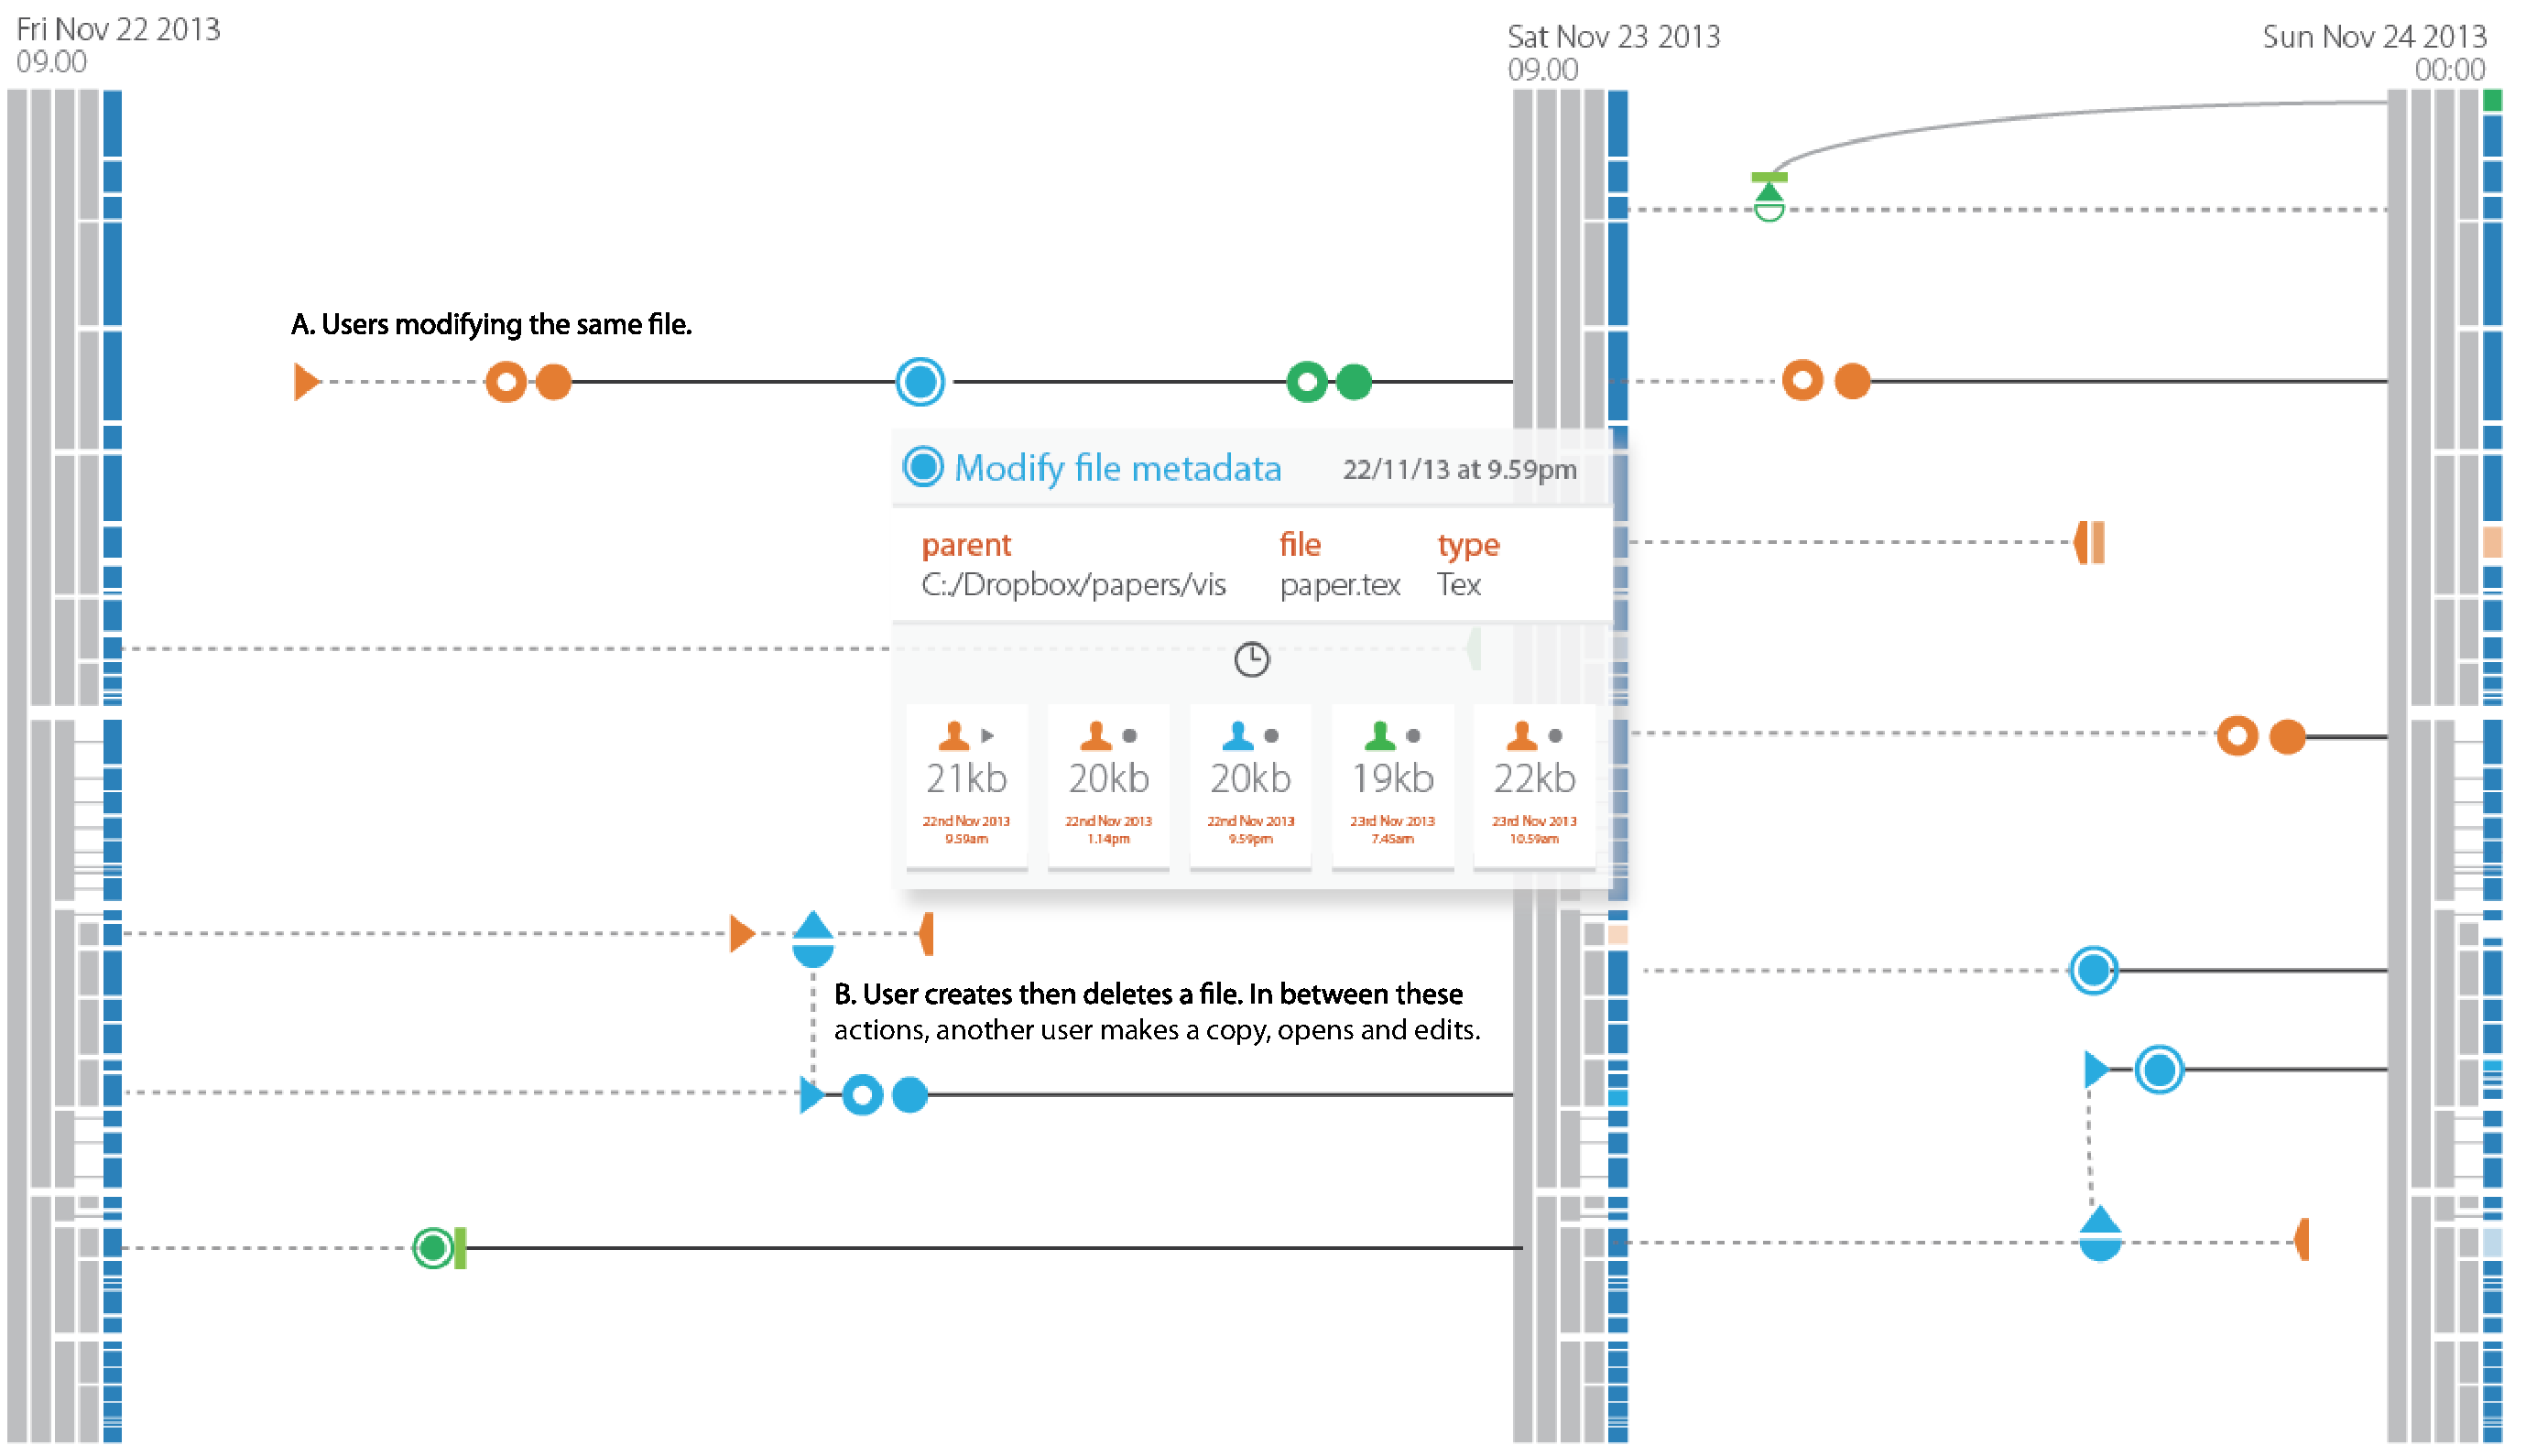
\includegraphics[width=\textwidth]{images/filesystem/dropbox-casestudy-2}
\end{center}
\caption{Glyph-based visualization is used to display events from a Dropbox activity log. The vertical bars are an abstract representation a directory tree and the timeline flows from left to right.
In event A) we can see the case where a number of users have been modifying the same file. The popup gives more details about the modifications, who did them and when. This allows for provenance tracking where such information is available.
In event B) we have another case where \emph{user X} (orange) creates a file, then \emph{user Y} creates a copy of this file, opens it and modifies its contents. \emph{User X} then deletes the original file, however a modified copy exists elsewhere.}
\label{fig:dropbox}
\end{figure*}

%
Dropbox is a popular cloud service that allows users to synchronise their files across multiple devices.
It allows users to create shared directories that other users can be invited to access.
This makes it especially useful for collaborative activities between institutions and colleagues, and for sharing personal media with family and friends.
Therefore it is desirable for users to visualise events in a shared folder, for instance, to see which file has been created or modified recently and by whom.
Although the service does provide a text-based activity log that users can access, it is time-consuming and tedious to read a long list of events.


As shown in Figure~\ref{fig:dropbox}, the glyph-based visualization allows users to gain an overview of the events in a shared folder.
As discussed previously, we avoided the use of colour in the initial glyph design.
This means that the visualization system can use this visual channel to encode additional dimensions, such as users or types of files.
In this example, colour is used to depict different three different users (shown in blue, orange, and green coloured glyphs).

The three vertical bars are simplified views of the directory tree concerned.
The period displayed spans over 39 hours, with a variety of events taking place.
Some indicate close collaboration, when a line of activities linked different users to a single file.
For example, the top line in the left section shows that the orange user created a file, and then opened and modified it.
After several hours, the blue user modified the metadata of the file (possibly renaming it or changing its access date).
Several hours later, the green user opened and modified it.
If a viewer wishes to inspect an event in detail, or simply forget the meaning of a glyph, he/she can simply hover the mouse over the glyph and a pop-up window will display details about the event and the file or directory concerned.
The detailed information includes the filename, the parent directory, and the file type.
It also shows file-specific history, such as the operations that each user performed and the file size after each operation.
Collaborative colleagues can become aware of ongoing actions, reducing the need to inform each other of every file access action via email.
